% !TEX root = ../main.tex
\chapter{Guide to Formatting Figure, Table and Formula}

\section{Guide to formatting figure}
\begin{figure}[!htp]
  \centering
  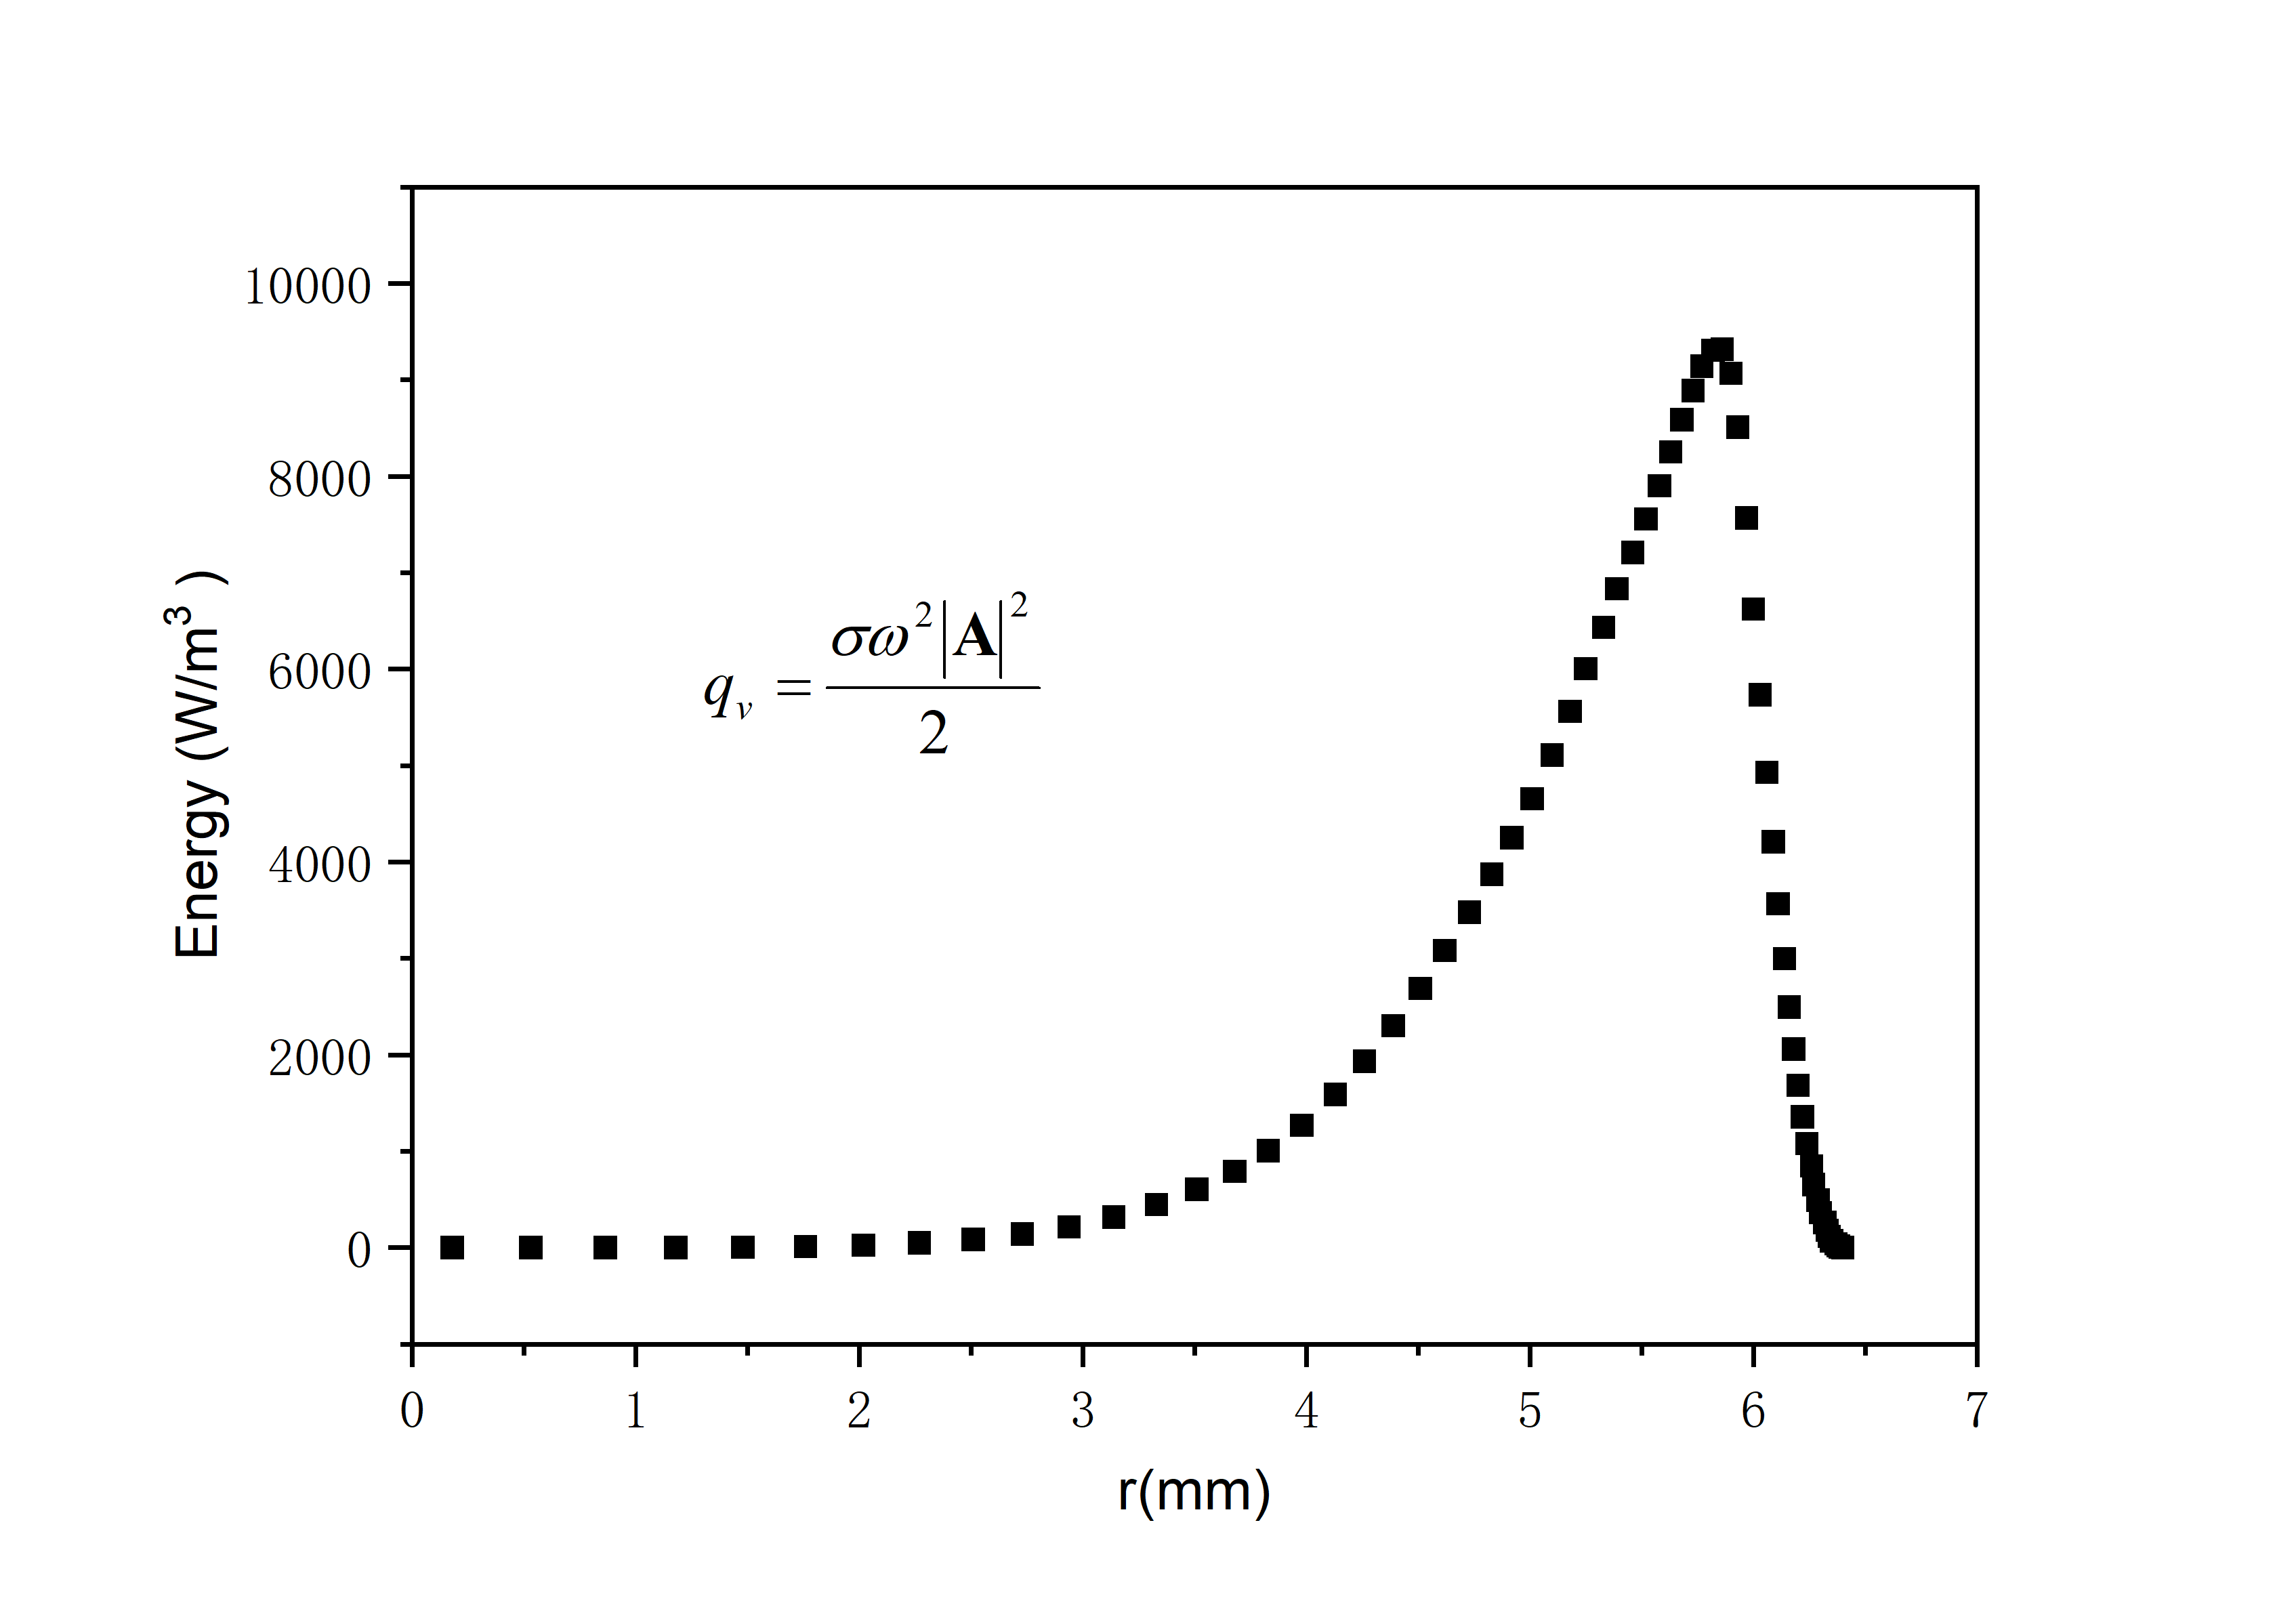
\includegraphics[width=8cm]{figures/energy.png} 
  \caption{XXX}
  \label{fig:energy}
\end{figure}

\begin{figure}[!hbtp]
  \centering
  \subcaptionbox{XXX}%
                [7cm]{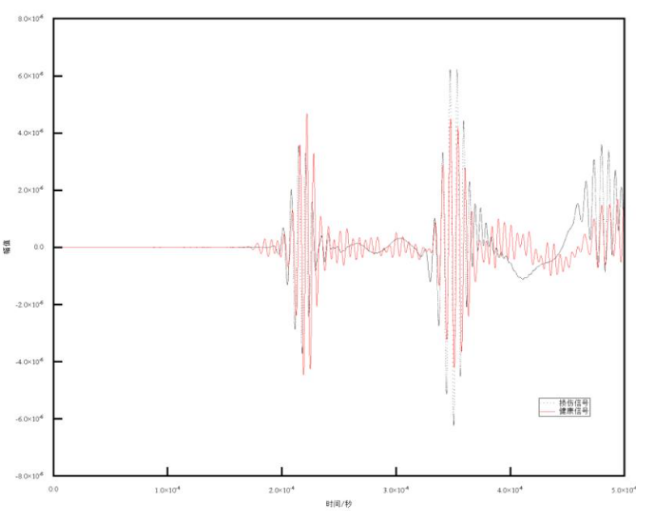
\includegraphics[height=6cm]{figures/signal_1.png}}
  \hspace{1cm}
  \subcaptionbox{XXX}%
                [7cm]{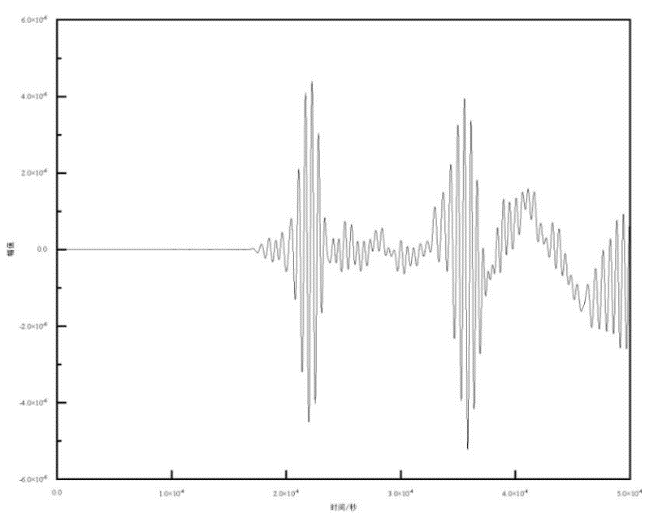
\includegraphics[height=6cm]{figures/signal_2.png}}
  \caption{XXX}
  \label{fig:bisubcaptionbox}
\end{figure}

\input{figures/mytable}

\section{Formula format}
\begin{equation}
 \frac{1}{\mu} \nabla^{2} \mathbf{A}-j \omega \sigma \mathbf{A}-\nabla\left(\frac{1}{\mu}\right) \times(\nabla \times \mathbf{A})+\mathbf{J}_{0}=0
\end{equation}


\section{Summary}
……
